\documentclass[12pt, a4paper, oneside]{report}
\usepackage[ngerman]{babel}
\usepackage{graphicx}
\usepackage{mathtools}
\usepackage{listings}
\usepackage{color}
\usepackage[citecolor=black, colorlinks=true, urlcolor=blue, linkcolor=black]{hyperref}

\definecolor{mygreen}{rgb}{0,0.6,0}
\definecolor{mygray}{rgb}{0.5,0.5,0.5}
\definecolor{mymauve}{rgb}{0.58,0,0.82}
\definecolor{amber}{rgb}{0.8, 0.5, 0.2}

    \title{\textbf{Biosphären Mess- und Überwachungsgeräte -- Funktionsprinzipien und Bedienungsanleitung}}
    \author{Tjark Gaudich}
    \date{November 2021}
    
    \addtolength{\topmargin}{-2cm}
    \addtolength{\textheight}{2cm}
\begin{document}
\lstset{basicstyle=\footnotesize, language=C, keywordstyle=\color{blue}, tabsize=4}

\pagenumbering{Alph}
\begin{titlepage}
\maketitle
\thispagestyle{empty}
\end{titlepage}
\pagenumbering{arabic}

\section{Vorwort}
Das folgende Dokument soll gleichzeitig als Dokumentation und Bedienungsanleitung für die Biosphären Umweltmessgeräte ("die Geräte") dienen, die ich für den Astrobiologie Projektkurs 2021/2022 bei Herr Krobbach entwickelt habe. Damit soll eine Nutzung und Wartung dieser Geräte weit über den Zeitraum meiner Schullaufbahn hinaus ermöglicht werden. Besonderer Fokus wird deshalb auf die Kommunikation mit dem PC zum Auslesen der Messwerte gelegt, da dieser vulnerabel für Änderungen des Betriebssystems ist, doch auch alle anderen Aspekte der Geräte sollen so sehr vertieft werden, dass sie ohne großes Vorwissen verstanden und repariert werden können. Sämtliche Quelldateien sind zusammen mit dieser Dokumentation auf 
GitHub\cite{Github} frei zugänglich.
\tableofcontents
\listoffigures

\chapter{Mechanik}

Mechanisch lassen sich die Geräte in vier Komponenten unterteilen:
eine Grundplatte (in \autoref{fig:Querschnitt} Dunkelgrau), an der alle andere Teile und das Glas der Biosphäre befestigt werden, eine Platine mit Sensoren im Inneren (nicht gezeigt) und die Hauptplatine (grün) außen sowie ein Deckel (hellgrau), der die Elektronik vor Beschädigungen schützt.
\begin{figure}[h]
	\centering
	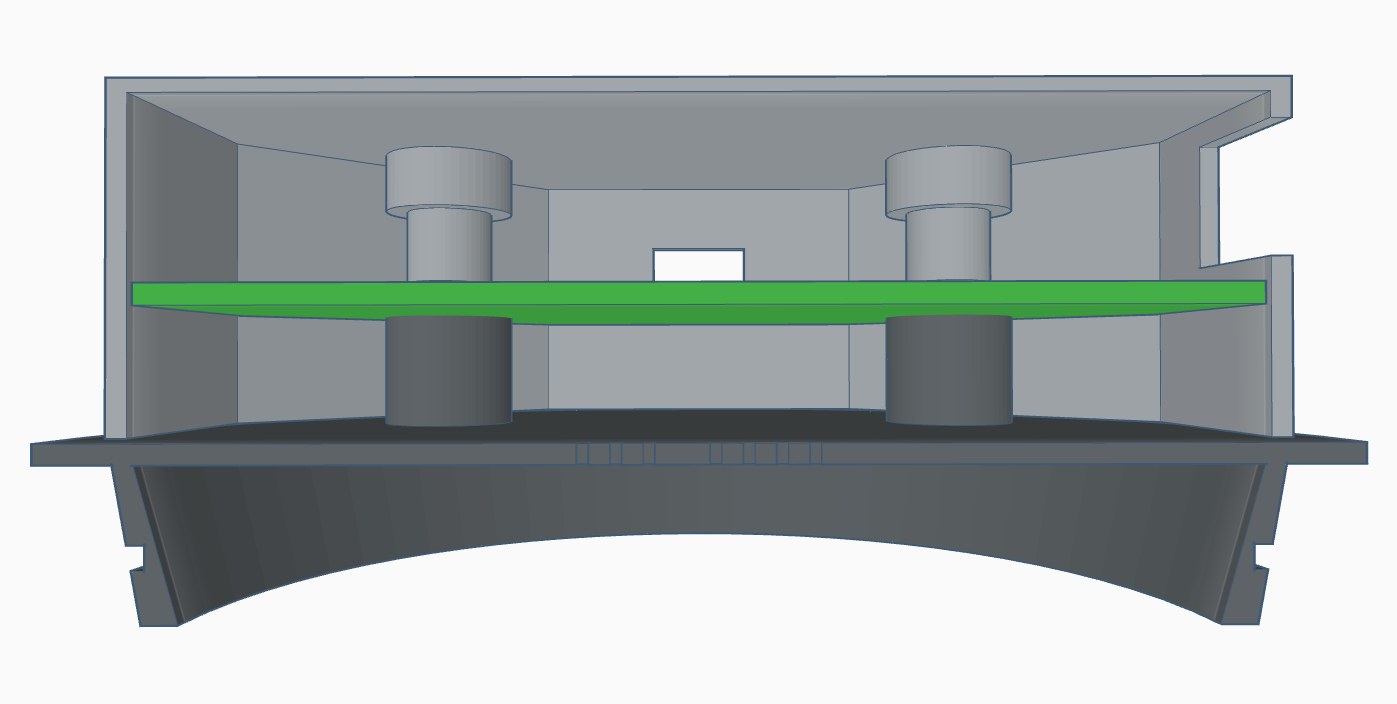
\includegraphics[width=1\textwidth]{pic/Querschnitt}
	\caption{Querschnitt durch das Gerät}
	\label{fig:Querschnitt}
\end{figure}
\\Auf die Platinen wird in \autoref{ch:elektronik} näher eingegangen, hier reicht es uns zu wissen das die unterer Platine nur über ihren Stecker befestigt wird und die obere ein Achteck von 85mm Durchmesser ist, vier Löcher mit je 50mm Abstand zueinander und 4mm Durchmesser zur Befestigung hat und 1,6mm Dick ist.

Deckel und Grundplatte sind beide aus PLA 3d gedruckt. Dabei wurde eine Auflösung von 0,2mm bei 100\% Infill verwendet
\section{Grundplatte}
Entsprechend dieser Maße ist die Oberseite der Grundplatte mit vier Röhren ausgestattet, in die M4 Einschraubmuffen montiert werden. Interessant ist jedoch die Unterseite, die in das Gurkenglas eingeklebt wird. Da die Luftmenge in der Biosphäre konstant ist kommt es bei Temperaturänderungen zu einer Druckänderung nach  dem Gesetz von Amontons \cite[S.~119]{Tafelwerk}, denen die Grundplatte und ihre Verklebung standhalten müssen. $p_0$ und $T_0$ sind dabei Druck und absolute Temperatur beim Verschließen der Biosphäre.
\begin{align}
\frac{p_0}{T_0} = \frac{p_1}{T_1} \footnote{}
\iff \Delta p = T  \times \frac{p_0}{T_0} - p_0
\label{eq:pressure}
\end{align}
Nehmen wir an, das die Biosphäre bei 20°C (293K) und Normaldruck verschlossen wurde und sich im Schlimmsten Falle auf 100°C (373K) aufgeheizt hat (darüber ist ihr Inhalt vermutlich tot, weshalb die Abdichtung irrelevant wird),
\begin{align}
\Delta p = 373K  \times \frac{1013hPa}{293K} - 1013hPa \approx 277hPa
\label{eq:pressure100C}
\end{align}
so ergibt sich nach \autoref{eq:pressure100C} ein Druckunterschied von 277hPa. Diese Druckfestigkeit mit einer Silikon Verklebung zu erreichen ist relativ einfach, beim Übergang zwischen Grundplatte und anschließendem Ring wird sie jedoch zu Herausforderung. Um eine höhere Festigkeit zu erreichen wurde dieser Übergang nach dem Druck zusätzlich mit einem Lötkolben verschmolzen. Diese Kombination hielt beim Anschließen eines Kompressors an einen Modifizierten Deckel etwa 300hPa Überdruck stand.

Falls sich zeigen sollte, das dies nicht ausreicht wäre eine Verdickung des Übergangs oder der Druck aus einem festeren Material, z.B.~Nylon, empfehlenswert.

Bei der Verklebung der Grundplatte mit dem Glas der Biosphäre sollte Aquariensilikon verwendet werden, da Sanitärsilikon für die Oranismen in der Biosphäre schädliche Zusatzstoffe enthalten kann.

\begin{figure}[h]
	\centering
	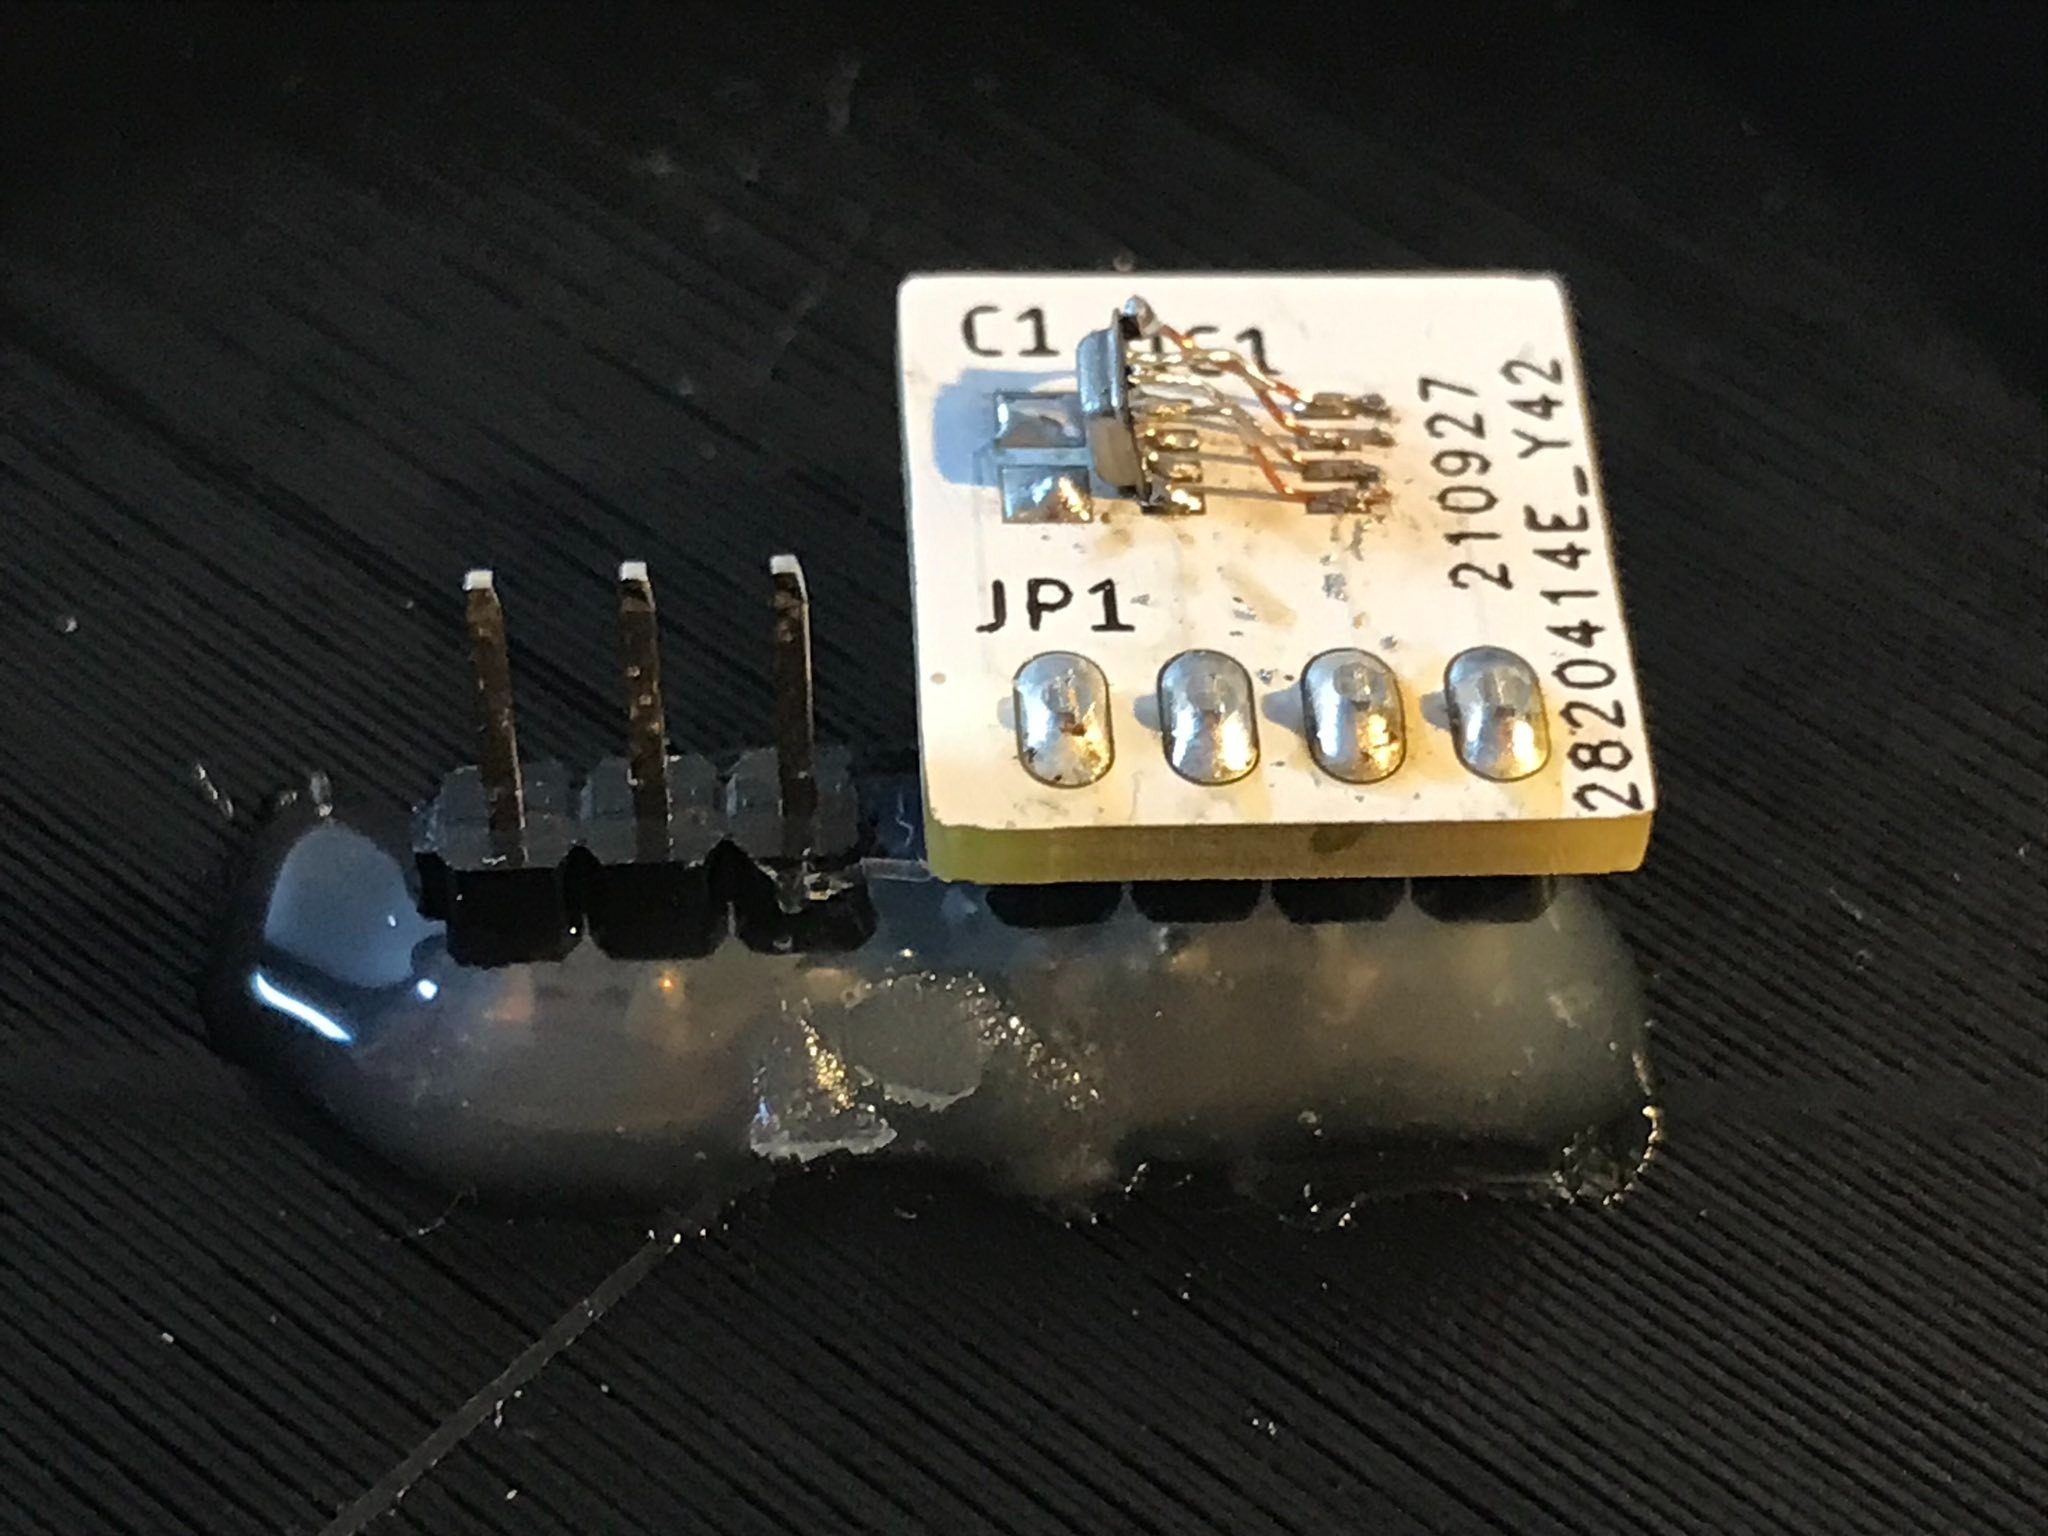
\includegraphics[height = 4cm]{pic/Stiftleisten}
	\caption{Fertig montierte Stiftleisten mit Sensorplatine}
	\label{fig:Stiftleisten}
\end{figure}

In der Platte befinden sich sieben Löcher, durch die Stiftleisten gesteckt werden um die Sensoren im Inneren mit der Hauptplatine zu verbinden. Dabei wird eine Stiftleiste von oben eingesteckt, mit Epoxidharz (UHU Endfest 3000) verklebt, von unten eine weitere Stiftleiste angelötet und die Lötstelle mit Heißkleber fixiert.

\section{Deckel}
Der Deckel besteht aus einem Achteck mit Abschlussplatte und eingesenkten Löchern, durch die er und die Hauptplatine mit vier M4~x~16 Schrauben an der Grundplatte befestigt werden. Beim Entfernen muss darauf geachtet werden, dass keine Kabel eingesteckt sind und der Deckel gerade nach oben abgezogen wird, um die durch ihn vorstehende Fotodiode nicht zu beschädigen.
\\
\begin{figure}[h]
	\centering
	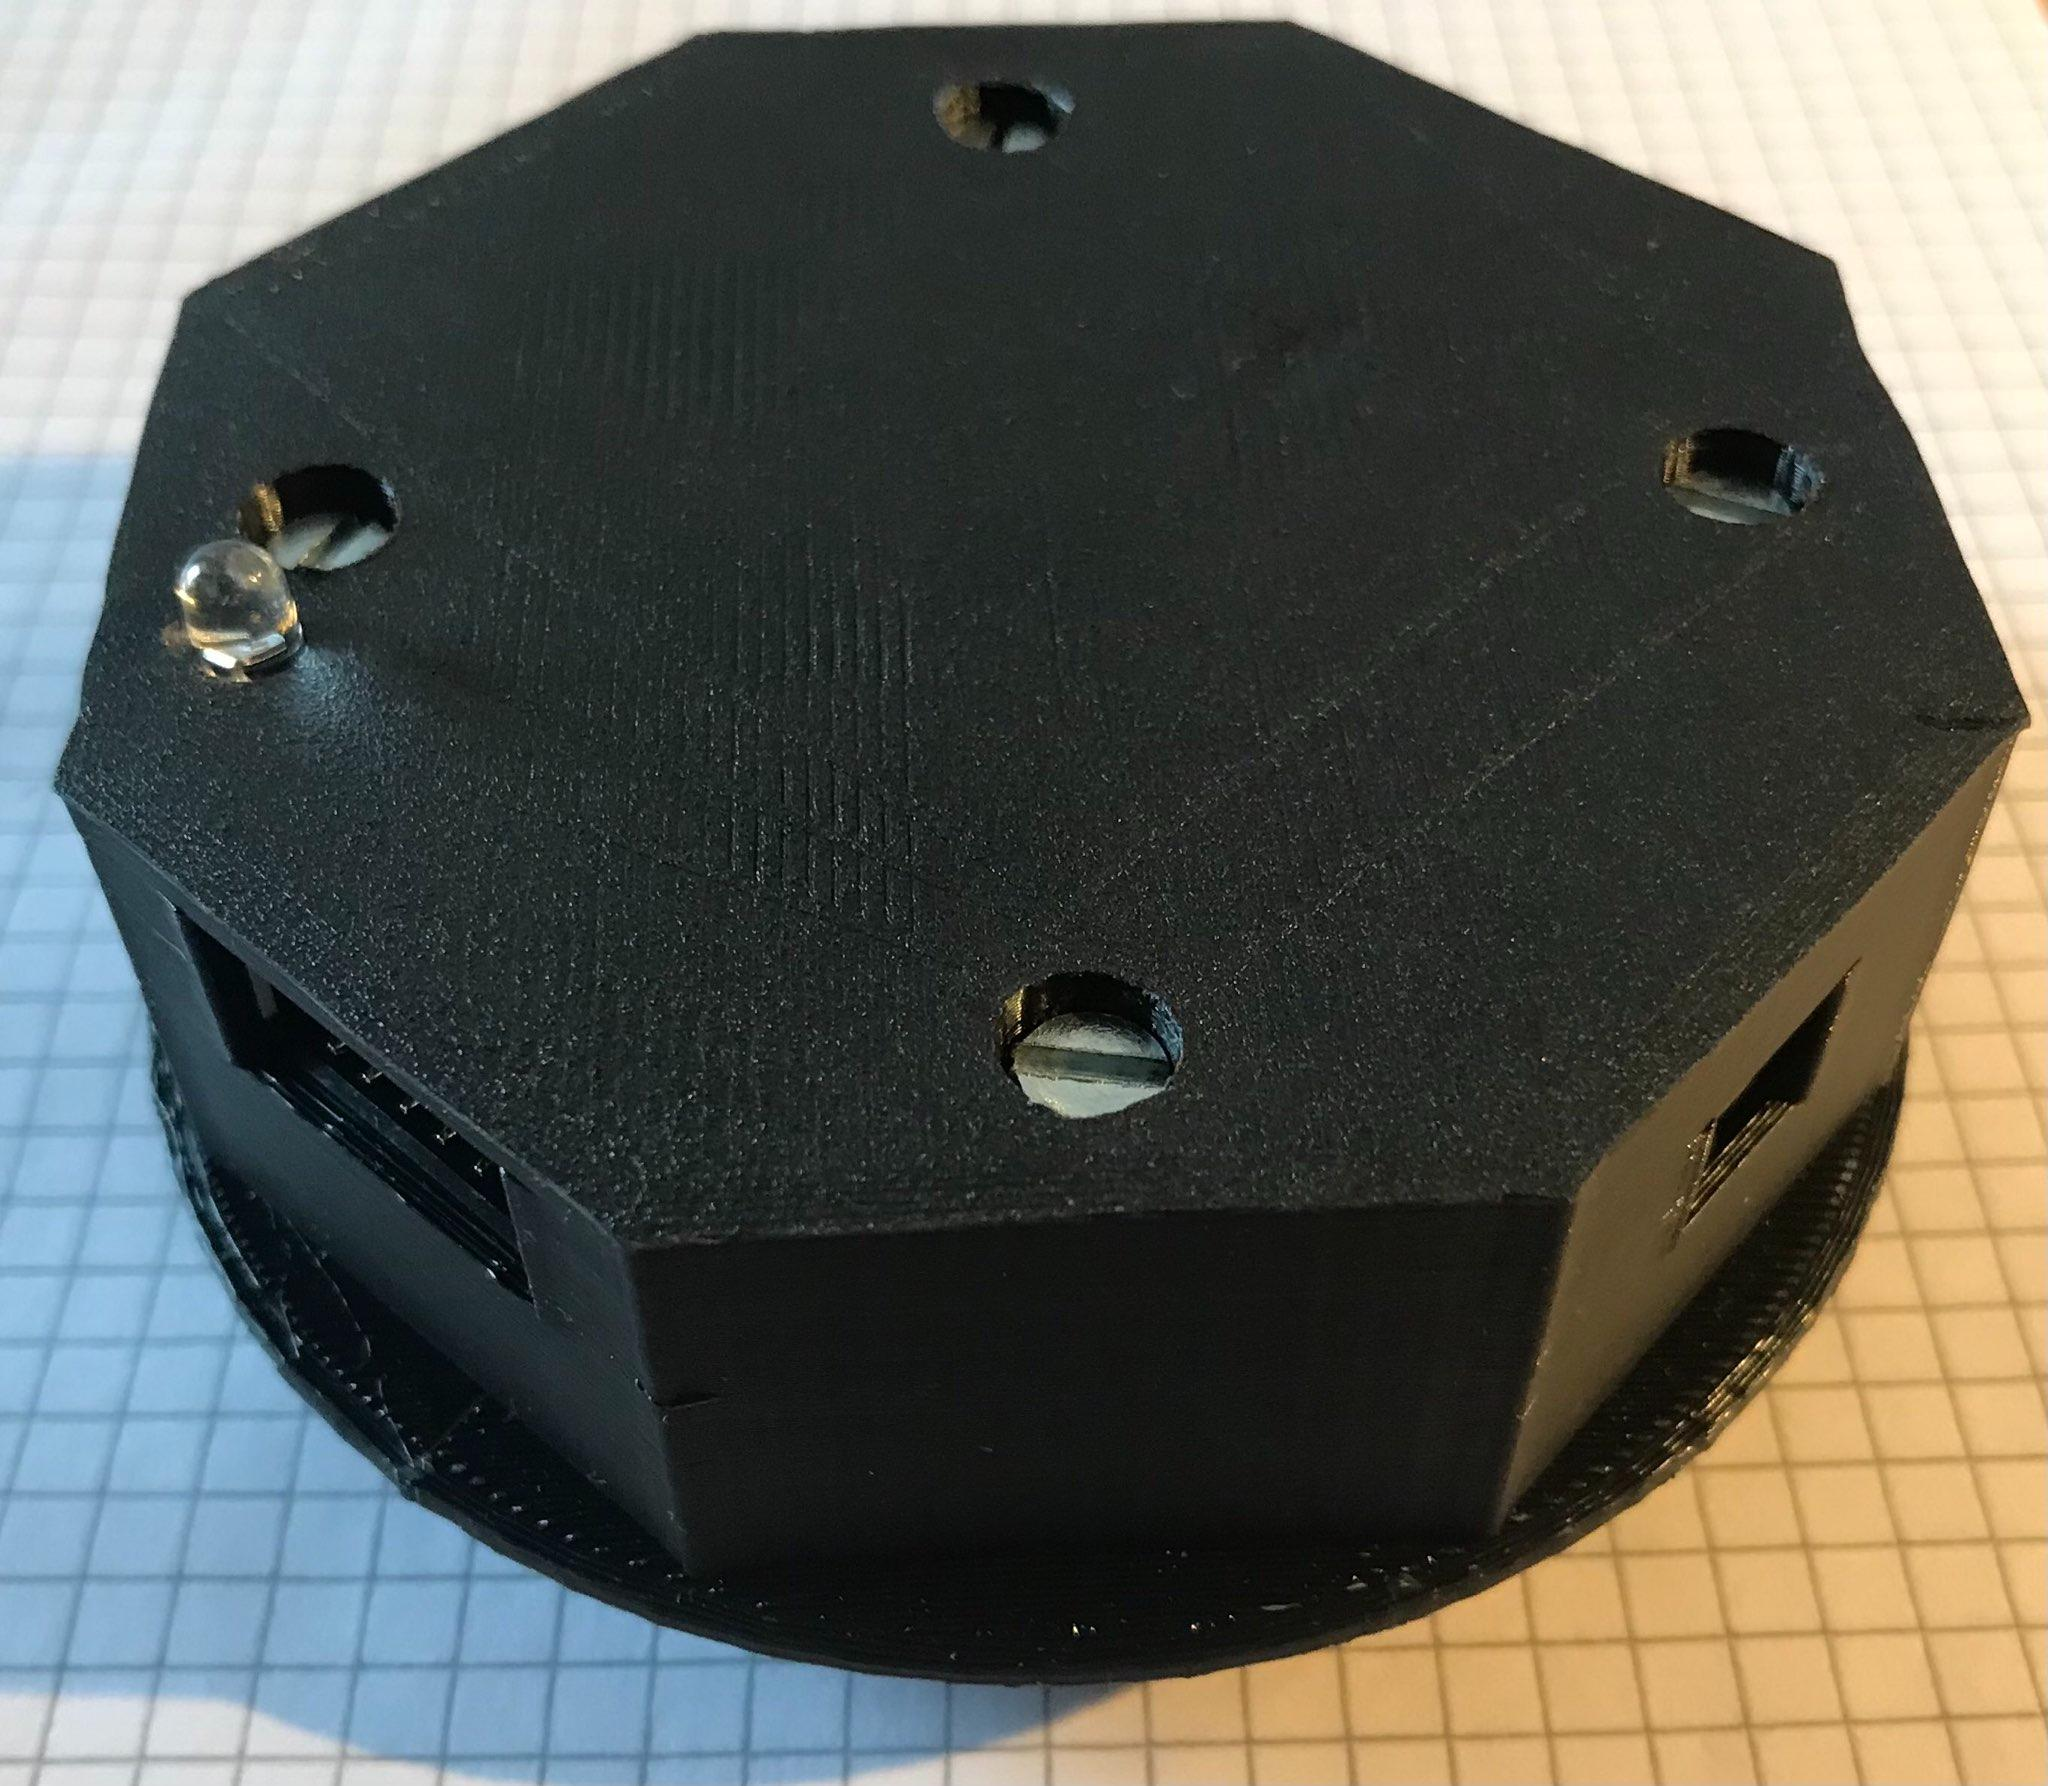
\includegraphics[width=0.7\textwidth]{pic/Komplett}
	\caption{Vollständig montiertes Gerät}
	\label{fig:Komplett}
\end{figure}

\chapter{Elektronik}
\label{ch:elektronik}
Die Elektronik besteht aus der Hauptplatine, die in fünf Funktionsblöcke unterteilt ist, einer Adapterplatine für den Luftsensor und einem ansteckbaren Bodenfeuchtigkeitssensor. Die Funktionsblöcke ensprechen den Seiten von "`biosphereMonitor.sch"', die Adapterplatine findet sich in "`Adapter.sch"'. Beide Schaltpläne und ihre dazugehörigen Platinen sind mit Eagle verfasst worden.

Eagle ist als Demoversion und für Bildungszwecke kostenlos und lässt sich unter \url{https://www.autodesk.de/products/eagle/free-download}\\ herunterladen.
\section{Mikrocontroller}
\label{sec:Mikrocontroller}
Alls Mikroncontroller findet ein ATxmega32A4AU\cite{ds:xmega} oder 16A4AU von Microchip Verwendung (IC1).

\begin{figure}[h]
	\centering
	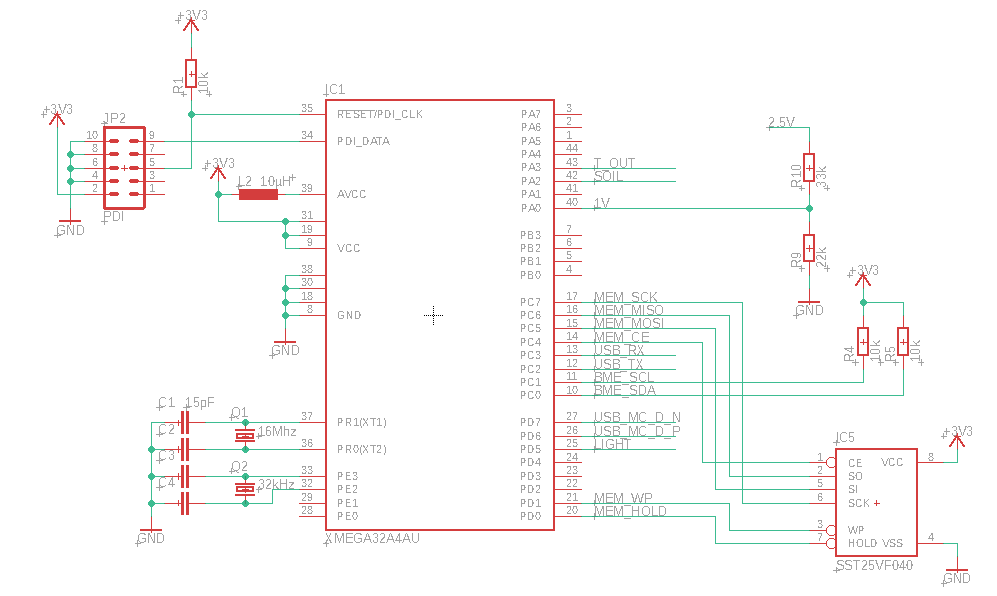
\includegraphics[width=0.9\textwidth]{pic/Microcontroller}
	\caption{Schaltplan Mikrocontroller}
	\label{fig:Microcontroller}
\end{figure}

\begin{figure}[h]
	\centering
\begin{tabular}{c|l}
	Pins & Funktion\\
	\hline
	10, 11 & TWI C, I²C Schnittstelle für den Luftsensoren 
	(\autoref{sec:Adapterplatine})\\
	12 (Tx), 13 (Rx)& UART0 zum USB UART Wandler (\autoref{sec:USB-UART Wandler}), \\&in Revision 1.0 vertauscht\\
	14 - 17 & Flash Spi Schnittstelle\\
	20, 21 & Flash Kontrollsignale\\
	25 & Lichtsensor (\autoref{sec:Außensensoren}), bei Steigender Flanke Pin Change Interuppt\\
	26, 27 & Reserviert für eingebautes USB\\
	32, 33 & Q2, 32.768kHz Uhrenquartz für die Realtimeclock\\
	34, 35 & PDI Programmierschittstelle\\
	36, 37 & Q1, 4 - 20MHz Hauptquartz, (16MHz Standard)\\
	40 & 1V Referenzspannung, über R9/10 aus 2,5V\\
	42 & ADC Eingang Bodenfeuchtigkeitssensor (siehe \autoref{sec:Bodenfeuchtigkeitssensor}) \\
	43 & ADC Eingang Temperatursensor (siehe \autoref{sec:Außensensoren})\\
\end{tabular}
	\caption{Pinbelegung Mikrocontroller}
\end{figure}
Dieser wird über die PDI Schnittstelle auf JP2 Programmiert. Das Pinout dieses Steckers ist kompaktibel mit dem des AVR ISP MK II Programiergeräts von Atmel/Microchip.
Die Frequenz von Q1 muss in $main.c$ und $makefile$ als F\_CPU eingetragen werden

Beim Flash handelt es sich um einen 4Mb 

\section{Stromverteilung}
\label{sec:Stromverteilung}

\section{USB-UART Wandler}
\label{sec:USB-UART Wandler}

\pagebreak
\section{Außensensoren}
\label{sec:Außensensoren}
Außen werden zwei Messwerte erhoben: Temperatur und Helligkeit.

Die Temperatur wird mit einem analogen Temperatursensor vom Typ LM35 \cite{ds:temp} der an TP6 eine Spannung von
$ 10mV * t~(in~^\circ C)$ anlegt. Diese wird vom Mikrocontroller (\autoref{sec:Mikrocontroller}) gemessen.

\begin{figure}[h]
	\centering
	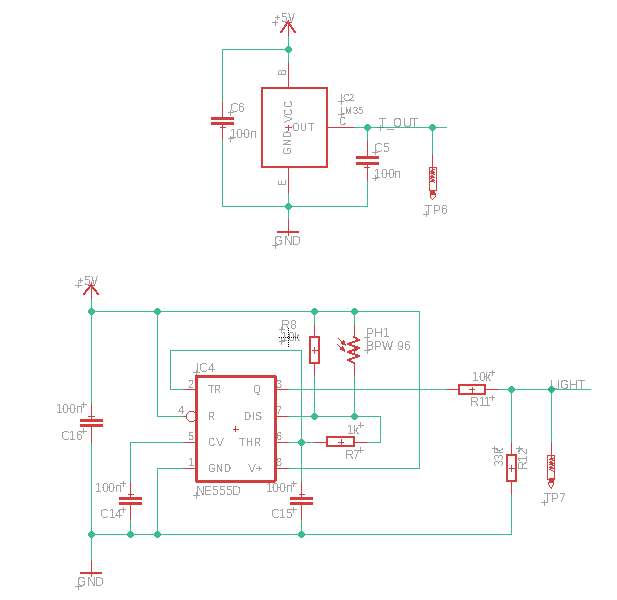
\includegraphics[width=0.8\textwidth]{pic/OutsideSensors}
	\caption{Schaltplan Außensensoren}
	\label{fig:Außensensor}
\end{figure}

Die Helligkeit wird mit einer Fotodiode vom Typ BPW96 \cite{ds:light} gemessen, die parralel zu R8 im Timingpfad des NE555 eingebaut ist. R11 und 12 teilen die Spannung des Ausgangssignales von 5V auf 3,3V, so das an TP7 ein 3,3V Rechtecksignal mit einer Frequenz exponential zur Lichteinstrahlung anliegt. Um die Einstrahlung zu bestimmen ist im Mikrocontroller eine Funktion fest einprogrammiert, die anhand der Messreihe aus $Lux~Messurments.ods$ bestimmt wurde. Die Formel hat das Format $f(x)=a \cdot x^b + c$. Um diese Formel zu füllen werden zunächst drei Punkte, erster, letzter und mittlerer aus der Messreihe, ausgewählt.

\begin{figure}[h]
\centering
\begin{tabular}{c|c|c}
	Nr. & x & y\\
	\hline
	1 & 1,27 & 0\\
	2 & 3,93 & 442\\
	3 & 6,21 & 1880\\
\end{tabular}
\end{figure}

Diese werden in \autoref{eq:lightB} bis \ref{eq:lightC} eingsetzt, um \autoref{eq:light} zu erhalten. Die dadurch erreichte Annäherung ist in \autoref{fig:Licht} oder $Lux~Messurments.ods$\footnote{\url{https://github.com/TjarkG/biosphere-monitor/blob/main/Documentation/Lux\%20Messurments.ods}} zu erkennen.

\begin{align}
y_3-y_1=\frac{y_2-y_1}{b^{x_2}-b^{x_1}}\cdot(b^{x_3}-b^{x_1}) \iff b \approx 1,65
\label{eq:lightB}
\end{align}

\begin{align}
a=\frac{y_2-y_1}{b^{x_2}-b^{x_1}} = 83,75
\label{eq:lightA}
\end{align}

\begin{align}
c = -a\cdot b^{x_1} + y_1 = -158,26
\label{eq:lightC}
\end{align}

\begin{align}
\label{eq:light}
f(x) = 83,75 \cdot 1,65^x -158,26
\end{align}

\begin{figure}[h]
	\centering
	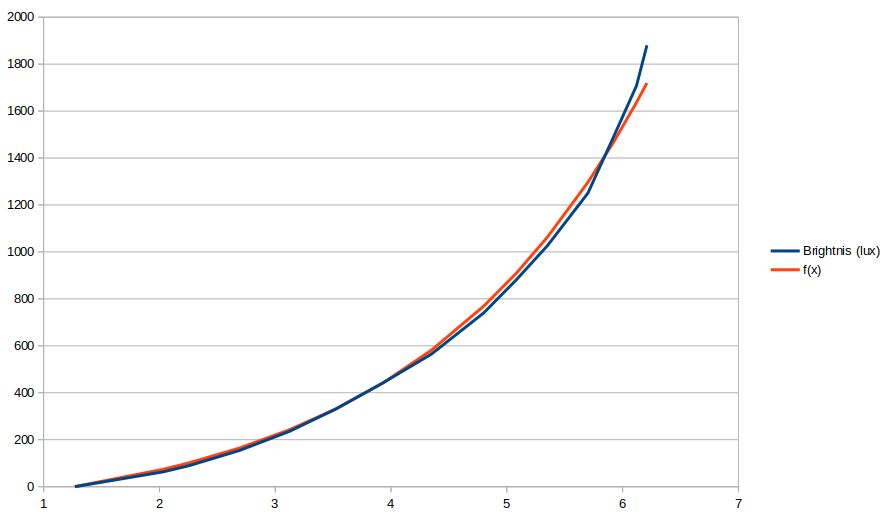
\includegraphics[width=\textwidth]{pic/Aproximation}
	\caption{Annäherung Messwerte}
	\label{fig:Licht}
\end{figure}

Dieser Werte sind auch in die Entsprechende Funktion in $main.c$\footnote{\url{https://github.com/TjarkG/biosphere-monitor/blob/main/Microcontroller/main.c}} eingesetzt
\begin{lstlisting}
unsigned int getLight(void)  //returns iluminace in lux
{
	if(lightFnom < 1200)     //Sensor cutoff Frequency
		return 0;
	return (unsigned int) ((66.46 * pow(1.732, (lightFnom/1000.0)) ) - 133.5);
}
\end{lstlisting}

\section{Anschlüsse Innensensoren}
\label{sec:Innensensoren}

\section{Adapterplatine}
\label{sec:Adapterplatine}

\section{Bodenfeuchtigkeitssensor}
\label{sec:Bodenfeuchtigkeitssensor}

\chapter{Software}
Die Software besteht aus zwei Teilen, dem Code für den Mikrocontroller und dem Ausleseprogramm für den PC. Um die eine installieren und die andere nutzen zu können müssen beide zunächst gecloned und ihre abhängigkeiten installiert werden. Die Befehle können für Debian Linux Varianten einfach kopiert werden, für andere Distributionen oder MacOS ist \lstinline|sudo apt-get| durch das lokale Eqvivallent zu ersetzen
\section{Instalation}
\label{sec:Instalation}
Sämtliche benötigte Software kann durch ausführen von
\begin{lstlisting}
/bin/bash -c "$(curl -fsSL 
https://raw.githubusercontent.com/TjarkG/biosphere-monitor/main/Shell/install.sh)"
\end{lstlisting}
Installiert werden. Der Script wurde unter Ubuntu und Alpine Linux getestet. Falls dies nicht funktioniert kann die Installation auch manuel durchgeführt werden:
Zum Clonen muss zunächst $git$ installiert werden.
\begin{lstlisting}
$ sudo apt-get install git
\end{lstlisting}
Dann kann das Repository gecloned
\begin{lstlisting}
$ git clone https://github.com/TjarkG/biosphere-monitor
\end{lstlisting}
Und in den neuen Ortnder gewechselt werden.
\begin{lstlisting}
$ cd biosphere-monitor
\end{lstlisting}
Um die PC Software compilen zu können ist außerdem GCC als Kompiler notwendig.
\begin{lstlisting}
$ sudo apt-get install gcc
\end{lstlisting}
Die aktuelle Version kann jetzt jeweils mit
\begin{lstlisting}
$ cc PC/biosphere.c -o PC/biosphere; ./PC/biosphere /dev/ttyUSB0 -r
\end{lstlisting}
kompilert und ausgeführt werden. 
\pagebreak

Um die Mikrocontroller Firmware aktualisieren zu können, werden neben der Hardware (\autoref{sec:Mikrocontroller})  eine ganze Reihe Hilfsprogramme benötigt. Eine Erläuterungen zu ihrer Funktion findet sich unter \cite{UbuntuAVR}
\begin{lstlisting}
$ sudo apt-get install avr-libc binutils-avr gcc-avr avrdude make
\end{lstlisting}
Das Upload der Firmware erfolgt mit
\begin{lstlisting}
$ make program -C ./Microcontroller
\end{lstlisting}

\section{Mikrocontroller}
\section{PC}
\section{Scripte}
Im Ordner $Shell$ befinden sich zwei Scripte:
$install.sh$ ist der installationsscript aus \autoref{sec:Instalation}. 
Dieser führt die selben Schritte aus die auch dort beschrieben sind, 
ermittelt allerdings von selber den verwendeten Paketmanager.

Des weiteren ist $kiosk.sh$ enthalten.
Dieser Script hohlt sich einmal pro Sekunde von $biosphere.c$ die aktuellen Messwerte für das Messgerät 
an $/dev/ttyUSB0$ und zeigt sie auf dem Terminal an.
\begin{thebibliography}{9}
\raggedright 

\bibitem{Github}
  Tjark Gaudich,
  \textit{Biospher Monitor},\\
  \url{github.com/TjarkG/biosphere-monitor}\\
  GitHub.com,
  2021
  
\bibitem{Tafelwerk}
  Prof.~Dr.~Lothar Meyer et al.,
  \textit{Das große Tafelwerk interaktiv 2.0},
  Cornelsen Verlag, Berlin,
  1. Auflage, 8. Druck 2018
  
\bibitem{ds:xmega}
  Microchip Technology Inc.,
  \textit{ATxmega32A4U datasheet},\\
  \url{www.microchip.com/downloads/en/DeviceDoc/ATxmega128-64-32-16A4U-DataSheet-DS40002166A.pdf}\\
  Microchip.com,
  2011-2020
  
\bibitem{ds:Flash}
  Microchip Technology Inc.,
  \textit{SST25VF040 datasheet},\\
  \url{www.microchip.com/downloads/en/DeviceDoc/20005051E.pdf}\\
  Microchip.com,
  2005-2020
  
\bibitem{ds:usb}
  Future Technology Devices International Limited,
  \textit{FT2323R datasheet},\\
  \url{www.ftdichip.com/wp-content/uploads/2020/08/DS_FT232R.pdf}\\
  ftdichip.com, 2020
  
\bibitem{ds:temp}
  Texas Instruments Incorporated,
  \textit{LM35 datasheet},\\
  \url{www.ti.com/lit/gpn/lm35}\\
  TI.com,
  1999-2017
  
\bibitem{ds:light}
  Vishay Semiconductors,
  \textit{BPW96 datasheet},\\
  \url{www.vishay.com/docs/81532/bpw96.pdf}\\
  vishay.com,
  2011
  
\bibitem{ds:BMP280}
  Bosch Sensortec GmbH,
  \textit{BMP280 datasheet},\\
  \url{www.bosch-sensortec.com/media/boschsensortec/downloads/datasheets/bst-bmp280-ds001.pdf}\\
  bosch-sensortec.com,
  Oktober 2021
  
\bibitem{ds:BME280}
  Bosch Sensortec GmbH,
  \textit{BME280 datasheet},\\
  \url{www.bosch-sensortec.com/media/boschsensortec/downloads/datasheets/bst-bme280-ds002.pdf}\\
  bosch-sensortec.com,
  Oktober 2021
  
\bibitem{ds:BME680}
  Bosch Sensortec GmbH,
  \textit{BME680 datasheet},\\
  \url{www.bosch-sensortec.com/media/boschsensortec/downloads/datasheets/bst-bme680-ds001.pdf}\\
  bosch-sensortec.com,
  Januar 2021

\bibitem{CLanguage}
  Brian W.Kernighan, Dennis M.Ritchie,
  \textit{The C Programming Language},
  Prentice Hall PTR, New Jersey,
  2. Auflage, 58. Druck 2018
  
\bibitem{UbuntuAVR}
  Ubuntu Wiki,
  \textit{AVR},\\
  \url{https://wiki.ubuntuusers.de/AVR/}\\
  Ubuntu Deutschland e.V.,
  Januar 2021

\end{thebibliography}

\end{document}